%!TEX root = ../main.tex

        \chapter{PPMS测量系统} % (fold)
        \label{cha:PPMS测量系统}
            器件的测量在PPMS(Physical Proerty Measurement System)中进行,为基础的二端微波测量。在PPMS中器件被冷却到2K左右,此时金属Nb进入超导态。通过网络分析仪直接测量二维平面波导的透射信号,即可在谐振腔的谐振频率处看到透射信号被吸收形成的凹陷。我利用现有的其他类型谐振腔对测量系统进行了测试,并通过拟合可得到谐振腔的相关参数。在测量系统搭建较为完善的基础上,进一步进行2.5维LC谐振腔的测量。通过对谐振腔的测量,可以验证理论计算所得的谐振腔频率是否与实验吻合,进而改进下一步的理论计算与器件参数设计。另一方面,通过测量谐振腔的品质因子,可以探究与减小谐振腔中的能量耗散,从而达到更好的通过与自旋耦合交换量子态的效果。

            \section{测量系统概述} % (fold)
            \label{sec:测量系统概述}

            实验中使用的网络分析仪为Agilent Technologies E5071C ENA series network analyzer,输出频率范围为300kHz至20GHz,下文中将简称其为VNA。


        \begin{figure}[h]
                \centering
            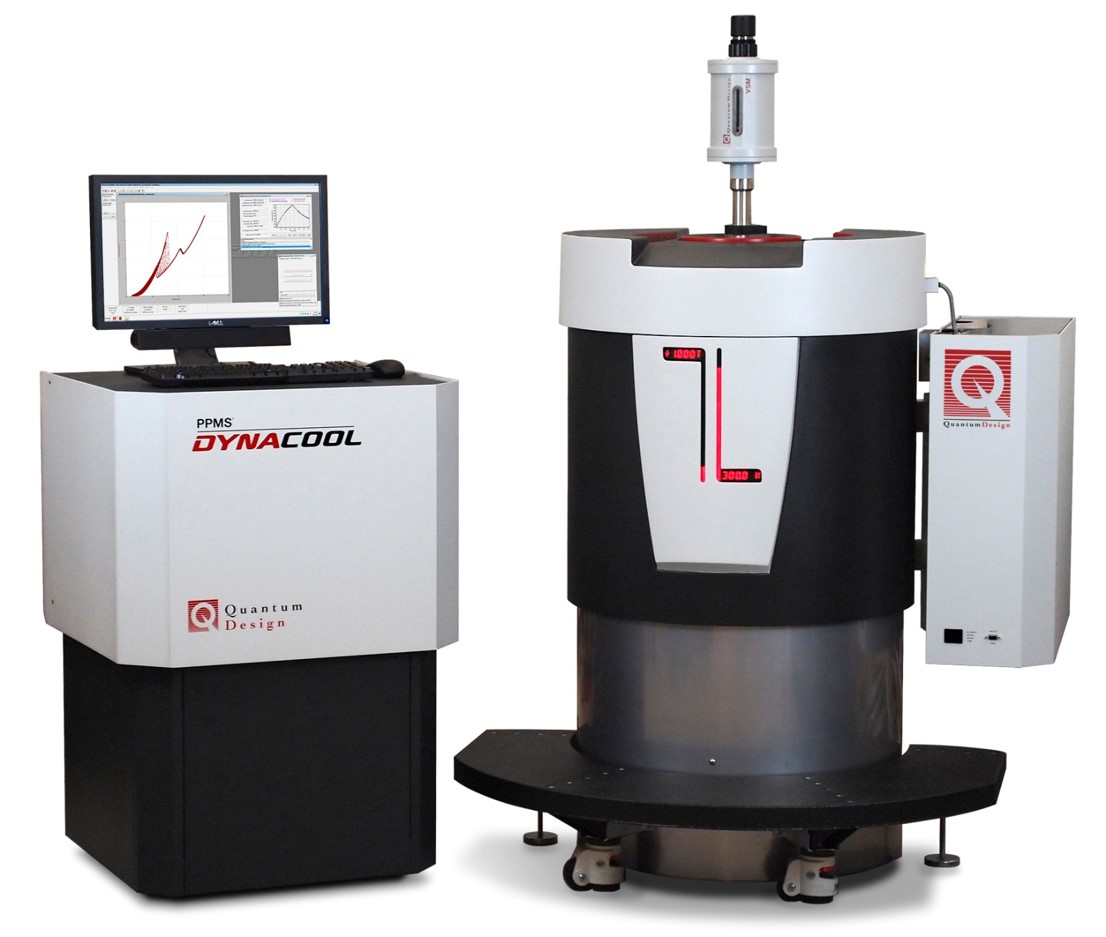
\includegraphics[width=4in]{DynaCool.jpg}
            \caption{PPMS DynaCool测量设备实物图\cite{QDDynaCool}}
            \label{fig:DynaCool}
        \end{figure}

            实验中所用的PPMS为QuantumDesign公司的DynaCool\cite{QDDynaCool},本文中都将简称它为PPMS。该PPMS可降温至1.8 K,加磁场最大为9T或14T,取决于磁体的型号。PPMS本体如图\ref{fig:DynaCool}所示,主要由控制电脑与仪器腔体两部分组成。仪器腔体的内部结构由图\ref{fig:DynaCoolStructure}所示。该图为仪器腔体在竖直平面内的横截面,可以看见样品室为被制冷环境包围住的一个立体圆柱形结构,直径不到一分米,有效的温度与磁场区域的高度大概在一分米左右。


        \begin{figure}[h]
                \centering
            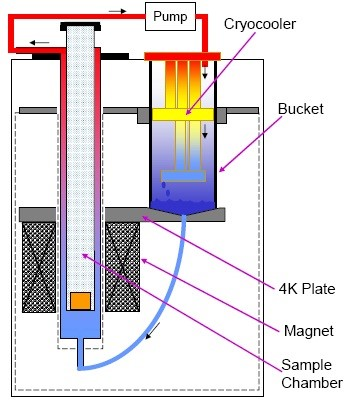
\includegraphics[width=4in]{PPMSStructure.jpg}
            \caption{PPMS DynaCool腔体内部结构\cite{QDDynaCool}}
            \label{fig:DynaCoolStructure}
        \end{figure}

            由于测量样品所在区域较小,因此无法进行需要很多端口的微波测量,但对于测量谐振腔性质所需的两个端口甚至一个端口来说较为合适。通过减小样品空间所取得的优点即在于,该PPMS系统的制冷系统长时间处于4K的低温,样品位于相对独立的样品室中,通过样品架与制冷系统的物理接触达到降温的效果,因此样品室可以较快地升温降温,而不需要对整个制冷系统进行升温降温。实际使用过程中,升温过程与降温过程所需时间均仅为30分钟左右,使得更换样品极为便捷。



            在开始本文的测量相关项目之前,该PPMS系统多用于直流测量,没有微波测量所需的设备。该部分设备的改造由交叉信息研究院孙麓岩研究组的郭星翰同学完成。改装后的样品通过样品托固定于样品杆上,进而通过样品杆插入PPMS的样品室中。由郭星翰设计的样品托如图\ref{fig:samplerodHolder}中蓝色矩形部分所示,由底座与盖子两部分组成。更换器件时,首先使PPMS样品室回到常温常压,取出样品杆,将样品托底座从盖子上拆下,再将旧样品从底座上取下,新样品安装上底座后将底座装回,插回样品杆即可。如图\ref{fig:samplerodHolder}所示,所测量的器件大小为4mm~x~7mm,放置于样品盒底座上的PCB板中央,通过点焊与PCB板相连。PCB板上焊接有两个SMP接头,与样品杆上的微波线相连并接入VNA的输入与输出端口。


\begin{figure}[h]
  \centering%
  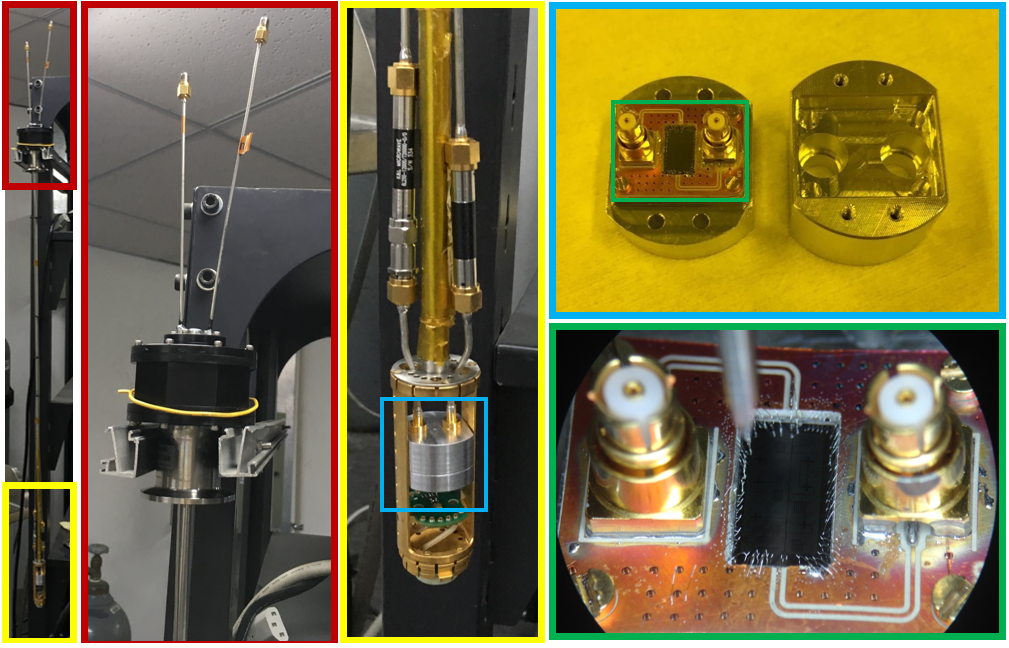
\includegraphics[width=\textwidth]{SampleRodAndHolder.png}
  \caption{样品杆与样品盒。其中红色矩形部分为样品杆末端微波信号的输入与输出端,黄色矩形部分为样品盒所处位置,蓝色矩形为样品盒以及拆卸后的样品盒。绿色矩形内为样品盒底座上的PCB板,SMP接头以及器件及其放大图}
  \label{fig:samplerodHolder}
\end{figure}

            在实验进行过程中,我们考虑到将来进行自旋与谐振腔耦合的相关实验时需要加入竖直方向的磁场以改变自旋能级间距,而现有设计下磁场垂直与器件表面,对超导态下的器件的性质影响较大。因此,我在现有样品托的基础上改进了样品托底座与盖子以及PCB板的设计,具体在第\ref{sec:样品托的设计与改进}节中详细进行描述。
                
            % section 测量系统概述 (end)

            \section{测量系统的程序编写} % (fold)
            \label{sec:测量系统}
            通过VNA测量谐振腔的频率响应时,需要调整VNA的输出功率,IFBW,扫描频率范围,平均次数等一系列参数。这些调整步骤既可通过仪器前面板的按钮进行,也可通过远程通讯来控制。考虑到测量的便捷性,我希望通过GPIB线与VNA进行通讯并取得数据。通过Agilent提供的GPIB-USB转接头建立硬件连接,并安装Keysight Instrument Control Bundle软件后,转接头上的工作指示灯正常。Keysight Instrument Control Bundle软件提供了Keysight IO Libraries Suite软件的安装与Command Expert软件的安装。前者能够方便地查看仪器的连接状态,后者则提供仪器的SCPI指令集并可测试通过指令控制仪器。

            通过电脑与VNA建立通讯后,我以MATLAB提供的visa类为基础,通过Command Expert对VNA的相关控制指令进行了测试后,编写了通过MATLAB控制VNA的代码,具体代码可在附录\ref{cha:measurement_code}中查看。对于能够简单进行更改与询问的参数,重载了MATLAB的get与set方法。对于大范围的精细的扫描,编写了manualSweep方法,可自动将扫描范围分段进行,并返回最终扫描结果。对于数据处理环节,我将拟合相关的代码也整合进入测量阶段,进而能够节省重新导入数据的过程直接快速得到拟合结果。使用MATLAB代码进行谐振腔的测量,在1个小时内即可完成大范围搜索谐振腔的共振频率位置,对不同频率的谐振腔进行细扫并拟合得到品质因子这一系列实验步骤。以下为一部分示例代码。大部分代码采用了inputParser处理输入参数,使程序规范且易于理解。

            \begin{lstlisting}
% Example of using class E5071C
vna = E5071C('address',6);	% initialize the instrument object with GPIB address 6
vna.plotTrace;				% fetch current trace on VNA and plot in a figure
vna.freqCenter				% query and display the center frequency
vna.freqSpan = 10e6;		% set the frequency span to 10MHz
[freqs, trace] = vna.manualSweep('start',1e9,'stop',10e9,'res',1e5);	% manual sweep from 1GHz to 10GHz with 0.1MHz resolution
vna.freqCenter = 3.021e9;	% set frequency center
vna.freqSpan = 1e6;			% set frequency span
vna.plotTrace('issavedata',true,'avg',10);	% wait for 10 averages and save data while fetching the trace
vna.fit('fitall',true);		% fit the data in the current figure
            \end{lstlisting}



            对于PPMS的控制,仪器商为这台仪器提供了配套的LabVIEW程序,可以通过.NET网络协议远程控制PPMS。仪器商所提供的LabVIEW程序基于一个动态链接库文件QDInstrument.dll实现控制功能。为了通过MATLAB控制PPMS,我尝试将LabVIEW程序的VI封装成dll文件,再通过MATLAB加载与调用其中的函数。但由于LabVIEW的单个VI都会首先与PPMS建立连接,因此导致MATLAB中每调用一次PPMS的状态查看或是设置函数,就会重新建立一次连接,使程序运行缓慢,并且导致多个client同时与PPMS控制电脑上的server保持连接,可能导致潜在的问题。综合考虑后,我决定直接调用仪器商编写LabVIEW程序所调用的dll文件。

            由于不清楚QDInstrument.dll文件中程序的构成与相关接口,而这些信息是调用其中的函数所必需的。通过查询,我使用了ILSpy对该dll文件进行了反编译,结合LabVIEW程序对该dll的使用方法,确定了在MATLAB中正确调用该dll文件的方法,并以它为基础编写了通过MATLAB控制PPMS程序的代码。需要注意的是,在MATLAB中的PPMS代码的构造函数中我一添加了加载该动态链接库的MATLAB指令,但每次重启MATLAB后初始化一个PPMS实例时总是会遇到MATLAB无法找到或识别dll中应有的命名空间的错误。目前较为确定的解决办法是每次重新启动MATLAB时,需在命令行(Command Line)中手动通过NET.addAssembly方法加载dll文件,随后初始化PPMS实例。这时MATLAB仍然会报错,但此时尝试手动在命令行中输入相关内容,通过使用TAB键能够发现MATLAB已经能够识别出dll中的内容。这时再初始化PPMS实例仍然会得到报错,必须在命令行中输入调用dll中的任意对象,比如输入\mcode{QuantumDesign.QDInstrument.QDInstrumentType.DynaCool}后回车,随后再初始化PPMS实例即可成功。以下为加载dll与控制PPMS的代码示例,完整的PPMS控制代码附在\ref{sec:ppms控制代码}中。

            \begin{lstlisting}
% Example of using class PPMS
NET.addAssembly('path\to\the\file.dll');	% load the dll
ppms = PPMS;				% This will get error message. See the constructor for more parameters
QuantumDesign.QDInstrument.QDInstrumentType.DynaCool; % nothing happened, but required
ppms = PPMS;				% This time it should work
ppms.temp					% query and print the temperature
ppms.field					% query and print the magnetic field
ppms.tempStatus				% query the temperature status. It will return a QuantumDesign.QDInstrument.TemperatureStatus object
ppms.tempStatusStr			% query the temperature status. It returns a string, such as 'Chasing', 'Stable', etc.
ppms.fieldStatus
ppms.fieldStatusStr			% similar as for temperature status
ppms.setTemp(300,'tempRate',10,'tempApproach','FastSettle');		% set temperature
ppms.setField(1000,'fieldRate',100,'fieldApproach','Linear');		% set field
            \end{lstlisting}

            有了以上测量程序的编写,即可完全通过测量电脑询问与控制PPMS的温度与磁场,以及调节VNA的相关参数并取得VNA的扫描数据。更进一步的,通过Windows的远程桌面可以远程连接到测量电脑,从而使测量变得更为便捷。实际中我们只需要在取出和放入样品时到PPMS设备附近,其余时间均远程进行控制与测量。







            \section{测量系统测试} % (fold)
            \label{sec:测量系统测试}
                  对于上述PPMS测量系统,我利用自己编写的测量程序利用现有常见的CPW谐振腔进行了一系列测量测试,说明测量系统工作良好。测试所用的器件为用于制备超导量子比特所需的平面传输线谐振腔,如图\ref{fig:PPMSSetupTestChip}所示。


            \begin{figure}[h]
                \centering
                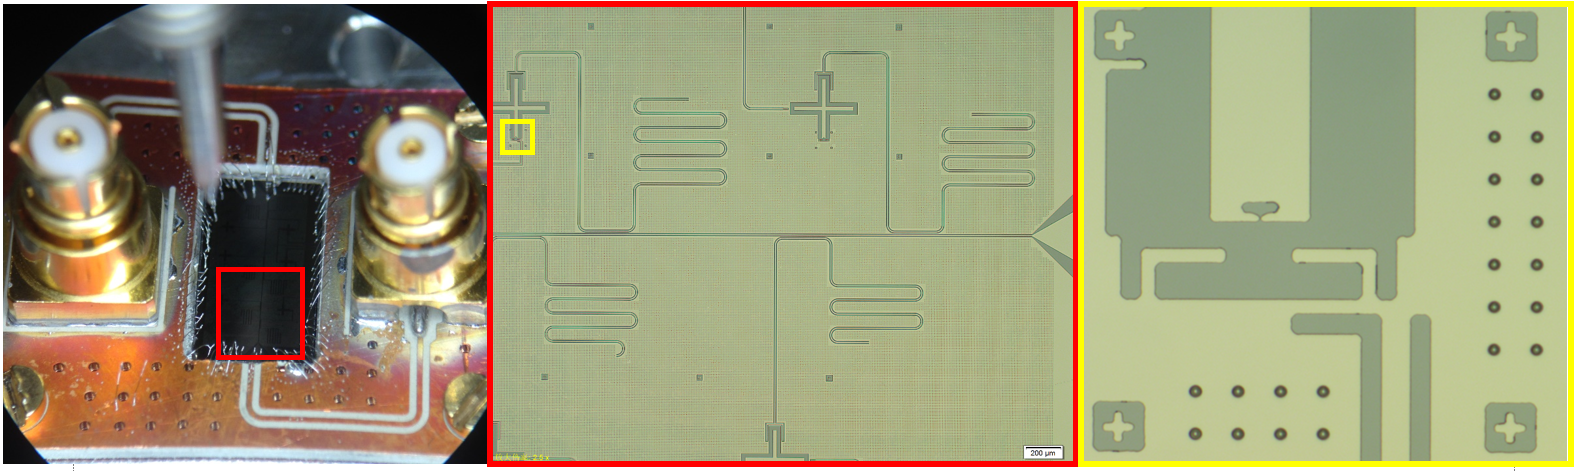
\includegraphics[width=\textwidth]{figures/PPMSTestChip.png}
                \caption{PPMS测量系统测试器件}
                \label{fig:PPMSSetupTestChip}
            \end{figure}

                  对于这种类型的平面波导谐振腔,已有较为详尽的研究\cite{Day2003,Wallraff2004Nature,schuster2007circuit,Gao2008Thesis,Barends2010APL,Geerlings2013},适合用于测量系统的测试。图\ref{fig:PPMSSetupTestChip}中左侧图即为样品底座的PCB板以及样品本身,红色矩形部分即为样品上的平面波导传输线以及从侧面与传输线耦合的平面波导谐振腔,即图\ref{fig:PPMSSetupTestChip}中部图片的S型部分。图\ref{fig:PPMSSetupTestChip}中部图片的深色区域为器件衬底,浅亮色区域为金属结构。黄色矩形区域即为超导量子比特关键的约瑟夫森节(J-J)所在区域,关于超导量子比特的基础知识将在附录\ref{cha:SCQubitPrinciple}中进行大致介绍。用于PPMS测量系统的测试仅需要谐振腔本身,因此超导节的区域并不需要制作J-J。最后,器件通过点焊与PCB相连,再通过PCB上的SMP接头接入PPMS测量系统。

                  利用超导量子比特系统所用的谐振腔,我对PPMS测量系统进行了基础的频率响应扫描,VNA输出功率的扫描,以及基于对PPMS系统的控制进行的温度与磁场的扫描。




                  \subsection{频率扫描} % (fold)
                  \label{sub:频率扫描}

                  频率扫描是测量谐振腔性质的基本方法。对于位于传输线内的电容耦合类型的谐振腔,其透射谱为谐振频率处透射增大的透射峰\cite{Wallraff2004Nature,schuster2007circuit},而对于挂在传输线侧面的谐振腔,也常被称为Hanger类型的谐振腔,传输线的透射谱在谐振频率出现透射降低的吸收峰\cite{Day2003,Gao2008Thesis,Geerlings2013}。在考虑最简单的忽略实际中可能出现的阻抗不匹配的情况下,测试所用的Hanger形式的谐振腔具有洛伦兹线型的吸收峰:

                  \begin{equation}
                  \label{eqn:simpleLorentzian}
                        |S_{21}|^2 = 1 - \frac{1/Q_r^2 - 1/Q_i^2}{1/Q_r^2 + 4 (f - f_r)^2/f_r^2} 
                  \end{equation}
                  其中$1/Q_r = 1/Q_c + 1/Q_i$为总品质因子,$Q_c$为耦合的品质因子,耦合越小其值越大,$Q_i$为本质的品质因子。对于更为复杂的情况,我们参考了文献\inlinecite{Megrant2012,Bruno2015,Geerlings2013}中使用的方法,拟合公式为\cite{Bruno2015}
                  \begin{equation}
                        \label{eqn:complexFitFunction}
                        S_{21} = A \left ( 1+ \alpha \frac{f-f_r}{f_r} \right ) \left (1- \frac{Q_l e^{i \theta}/|Q_e| }{1 + 2i Q_l \frac{f-f_r}{f_r} } \right )e^{i ( \phi_v f + \phi_0 ) }
                  \end{equation}
                  对该公式的推导与意义在参考文献\inlinecite{Bruno2015}中有所介绍。
                  

                  对于实际测量,往往需要进行大范围扫描找到谐振频率后再在谐振频率附近细扫。由于VNA频率采样点数有最大值,因此我编写了测量程序,在给定扫频范围与精确度下自动控制VNA分段扫描,并最后汇总数据,使大范围的精细扫描十分便捷。找到谐振模式后,在模式附近进行了细扫,并基于复杂情况的谐振腔响应公式,对测量所得的信号进行了拟合。测试过程中测得的典型数据如图\ref{fig:PPMSSetupTestFreqSweep}所示。
                  
                        
            \begin{figure}[h]
                \centering
                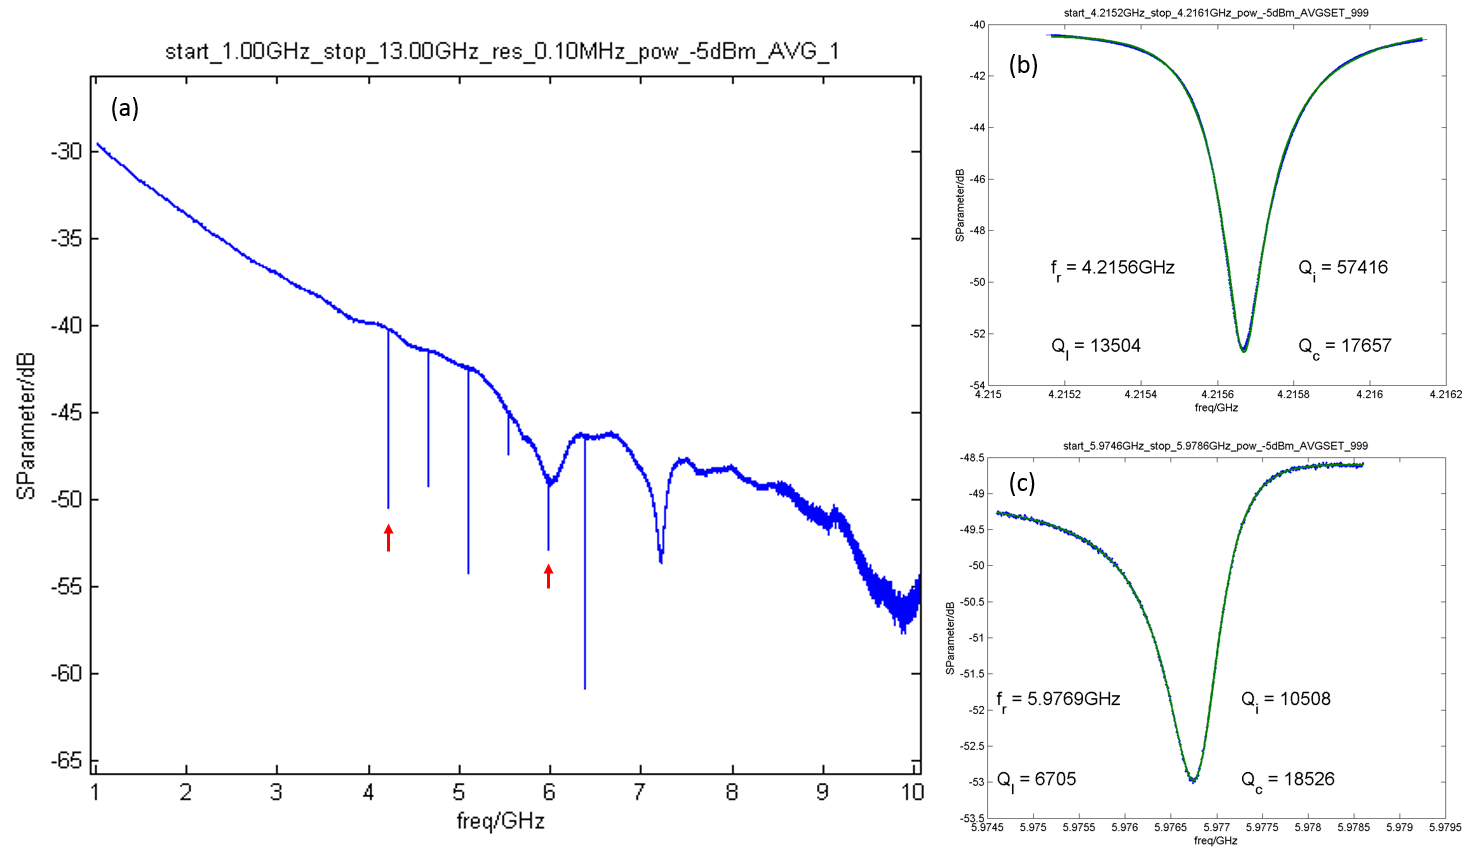
\includegraphics[width=\textwidth]{PPMSSetupTestFreqSweep.png}
                \caption{VNA频率扫描与拟合}
                \label{fig:PPMSSetupTestFreqSweep}
            \end{figure}

            通过大范围的扫描能够十分容易地确定谐振频率的位置,并获得测量系统的透射背景。通过根据所估计的器件谐振腔的$Q$值来调整大范围扫描的精度,可以避免因为精度过差而漏掉谐振模式的情况。图\ref{fig:PPMSSetupTestFreqSweep}(b)与(c)为(a)中红色箭头所示的谐振模式的透射曲线的拟合结果图。通过拟合能够得到该模式的$Q_i$,$Q_c$,谐振频率$f_r$等一系列参数。通过曲线可以看出,拟合得到的理论曲线(绿色实现)与实际数据(蓝色数据点)符合很好。对于如图\ref{fig:PPMSSetupTestFreqSweep}(c)中由于阻抗不匹配导致的非对称的响应线型,复杂情况下的通用公式也能拟合得到很好的结果。

                  % subsection 频率扫描 (end)


                  \subsection{VNA功率扫描} % (fold)
                  \label{sub:vna功率扫描}

                  在频率扫描的基础上,我继续编写了VNA的功率扫描的程序。通过以不同的功率测量谐振腔,能够观察谐振腔相关参数随功率的变化\cite{Day2003,Gao2008Thesis},对于用于读取超导量子比特状态的谐振腔而言,扫描功率的测量也是获得谐振腔本征频率与谐振腔和超导量子比特耦合强度参数的必要方法\cite{Blais2004,Blais2007,schuster2007circuit}。功率扫描的测量结果如图\ref{fig:PPMSTestPowerSweep}所示。


\begin{figure}[h]
  \centering%
  \begin{subfigure}{0.4\textwidth}
    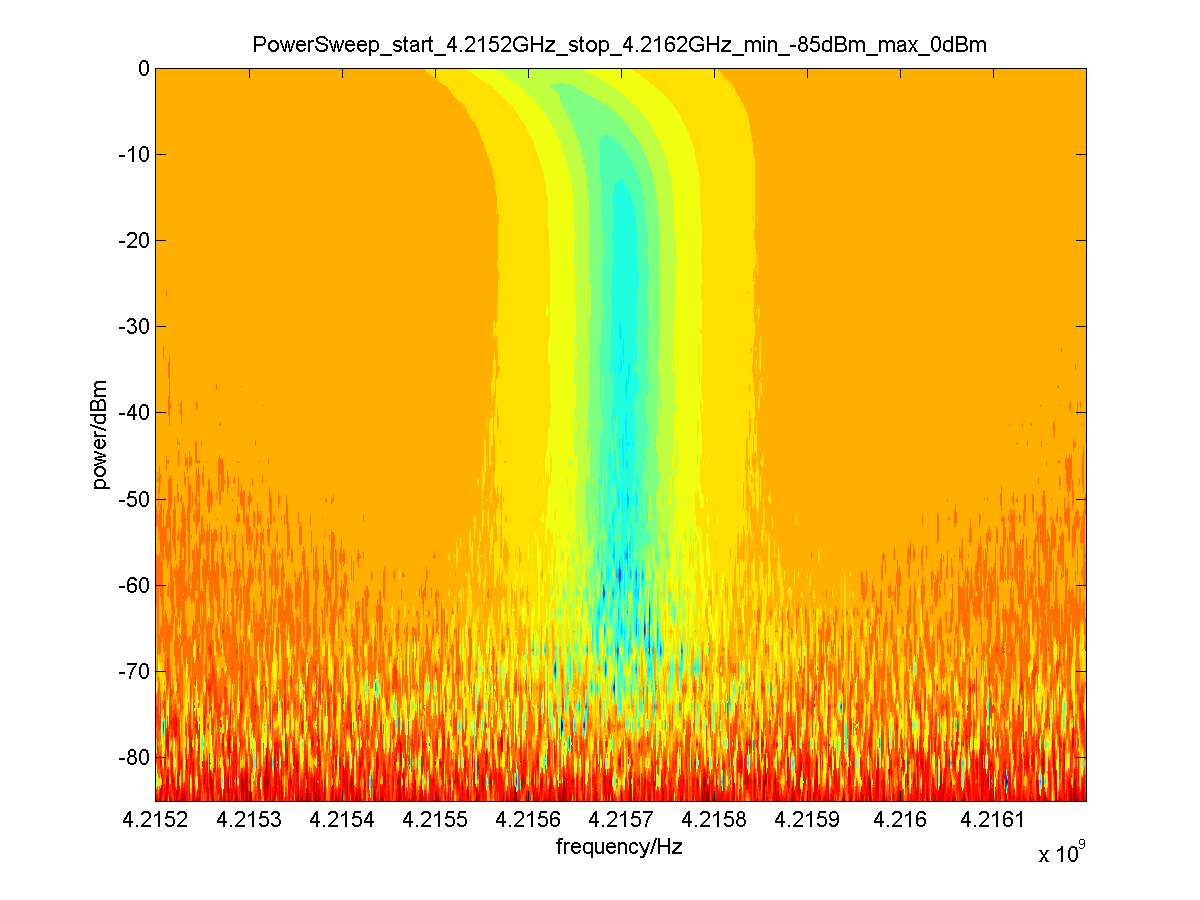
\includegraphics[width=3.2in]{figures/meas/Test_PowerSweep_start_4.2152GHz_stop_4.2162GHz_min_-85dBm_max_0dBm.png}
    % \caption{第一个小图形}
  \end{subfigure}%
  % \hspace{4em}%
  \hspace*{\fill}
  \begin{subfigure}{0.4\textwidth}
    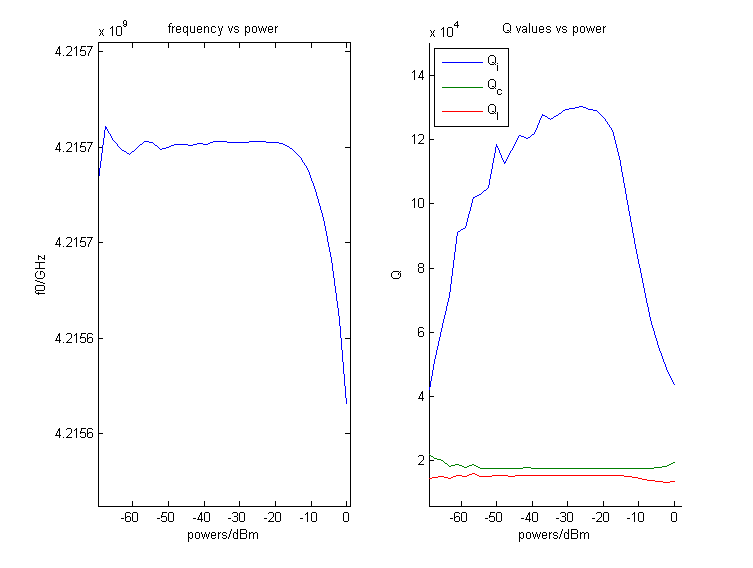
\includegraphics[width=3.2in]{figures/meas/Test_PowerSweep_freq_Q_vs_power_20170526T104027.png}
    % \caption{第二个小图形,注意这个图略矮些。subfigure中同一行的子图在顶端对齐。}
  \end{subfigure}
  \caption{VNA频率与功率扫描扫描}
  \label{fig:PPMSTestPowerSweep}
\end{figure}

                  
                  图\ref{fig:PPMSTestPowerSweep}中左图为透射率关于频率和磁场的关系图,透射率的大小通过颜色表示。能够明显看出功率较小时由于噪声较大,无法看出明显的吸收峰。随着功率的增大,逐渐能够看出谐振腔的吸收峰,并在功率较大时能够肉眼可见地看到频率与线宽的变化。图\ref{fig:PPMSTestPowerSweep}的右图为通过拟合后得到的谐振腔频率与品质因子随功率的变化。对于谐振腔的频率,在功率小于-20dBm时均没有明显变化,在功率很小时由于拟合的原因有所波动。在同样的功率区间内,$Q_i$随功率的增加而增加,其原因为更大的功率使谐振腔中引起耗散的杂质系统达到饱和,从而耗散减小,使得谐振腔的本征品质因子上升,与文献相符\cite{Barends2010APL,Megrant2012,Bruno2015}。当功率进一步增加时,谐振腔的频率发生红移,并且本征品质因子开始下降,导致这种现象的原因为功率进一步增加时激发了非超导态的准粒子,将对谐振腔的等效电感与电阻产生影响,相应地影响谐振腔的频率与耗散大小\cite{Day2003}。温度的升高也会激发更多的准粒子,因此在随后扫描温度的实验中我们也能观察到类似的现象。$Q_c$由耦合导致,手工率关系影响较小,与物理图像相符,而总的品质因子也由于主要受$Q_c$的限制而随功率变化不大。
                        
                  % subsection vna功率扫描 (end)

                  \subsection{温度扫描} % (fold)
                  \label{sub:温度扫描}

                  通过控制PPMS的温度,我们能够在不同温度下探究所测系统的特性。图\ref{fig:PPMSTestTempSweep}为对测试器件进行温度与频率扫描的结果。


\begin{figure}[h]
  \centering%
  \begin{subfigure}{0.4\textwidth}
    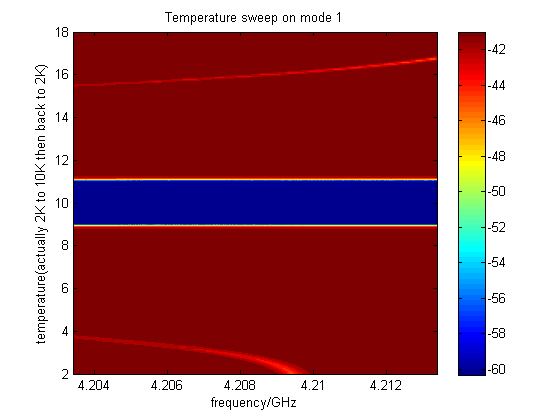
\includegraphics[width=3.2in]{figures/meas/Test_TempSweep20170513v2.png}
    % \caption{第一个小图形}
  \end{subfigure}%
  % \hspace{4em}%
  \hspace*{\fill}
  \begin{subfigure}{0.4\textwidth}
    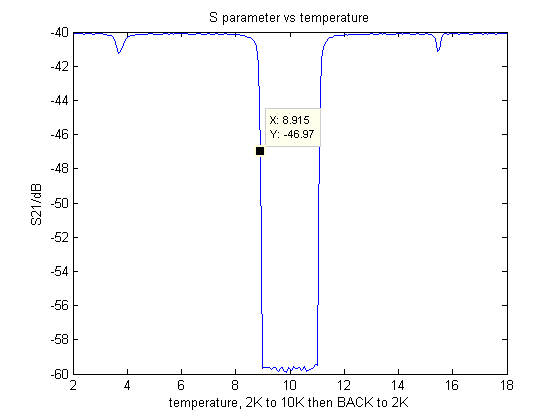
\includegraphics[width=3.2in]{figures/meas/Test_S_vs_T.png}
    % \caption{第二个小图形,注意这个图略矮些。subfigure中同一行的子图在顶端对齐。}
  \end{subfigure}
  \caption{PPMS温度与VNA频率扫描}
  \label{fig:PPMSTestTempSweep}
\end{figure}
                 
                 图\ref{fig:PPMSTestTempSweep}的左图为透射率关于频率与温度的变化图,透射率的单位为dB。频率在一个共振模式的附近扫描,而温度的扫描为从2K逐渐升高至10K再逐渐降低至2K,由于MATLAB画图的限制,纵轴的后半段为10K至18K,对应实际温度的由10K降低至2K。通过扫描温度的实验结果,能够明显看到两个现象。首先谐振腔的频率随温度的上升而红移,并且线宽变宽,峰的大小变浅,与功率较大时进一步增大功率时观察到的现象相符,同样说明了这种变化趋势可通过准粒子的增加进行解释。另一方面,在温度增加到8.9K附近时,整个透射率的背景十分迅速地下降了近20个dB,能够确信地得出观察到了器件失去超导性质这一结论。通过测量得到的Nb薄膜的超导临界温度$T_c=8.9$K也与经验相符,略低于实体Nb的超导温度$9.25$K\cite{cardarelli2008materials}。
                        
                  % subsection 温度扫描 (end)

                  \subsection{磁场扫描} % (fold)
                  \label{sub:磁场扫描}

                  在自旋与谐振腔耦合的实验中,通过磁场调节自旋系统的能级结构是十分常见的实验操作\cite{kubo2010,PhysRevA.95.022306,Bienfait2016a}。因此我编写了控制PPMS的磁场的程序,并通过测试器件进行了扫描频率与磁场的测试,测量结果如图\ref{fig:PPMSTestFieldSweep}所示。


\begin{figure}[h]
  \centering%
  \begin{subfigure}{0.4\textwidth}
    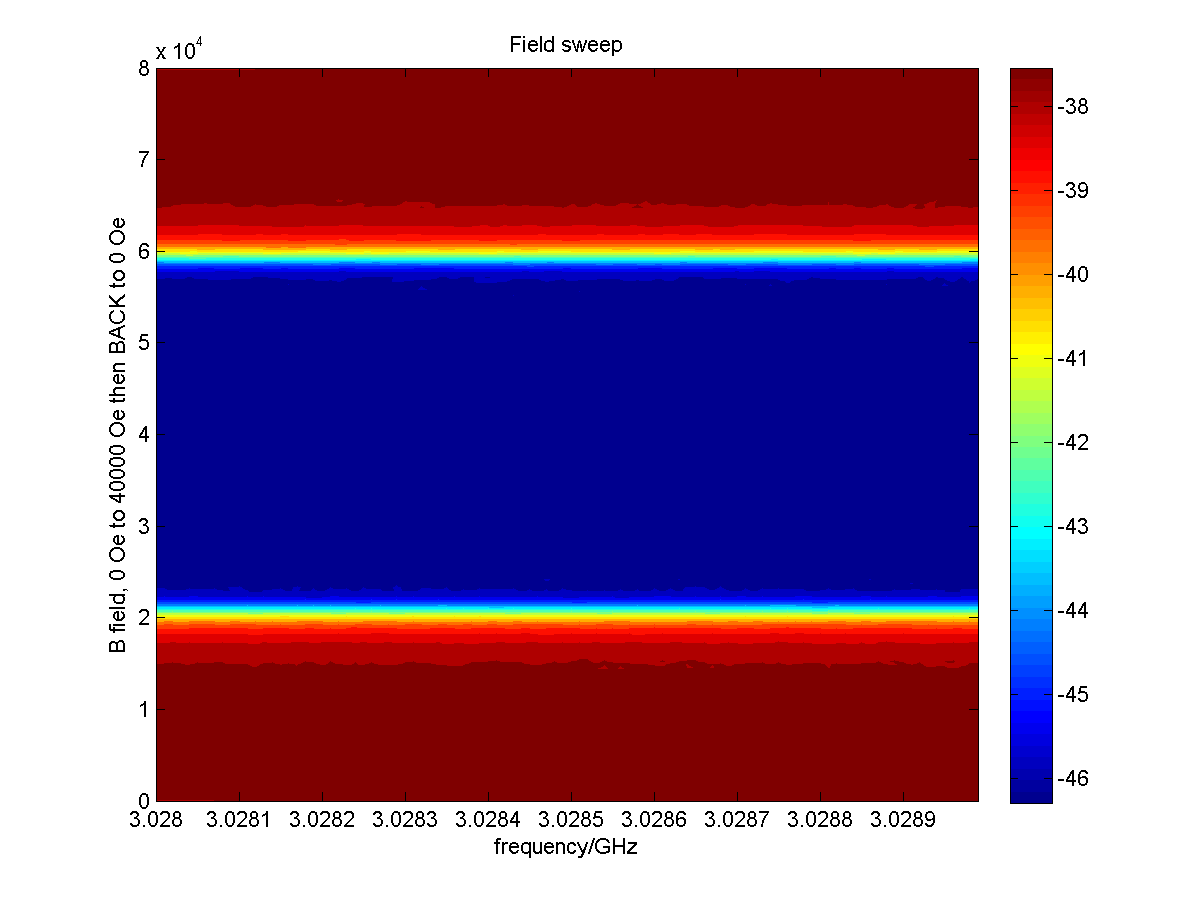
\includegraphics[width=3.2in]{figures/meas/Test_FieldSweep_start_3.0280GHz_stop_3.0290GHz_pow_-10.0dBm_minB_0G_maxB_40000G_numB_200_20170517T112932.png}
    % \caption{第一个小图形}
  \end{subfigure}%
  % \hspace{4em}%
  \hspace*{\fill}
  \begin{subfigure}{0.4\textwidth}
    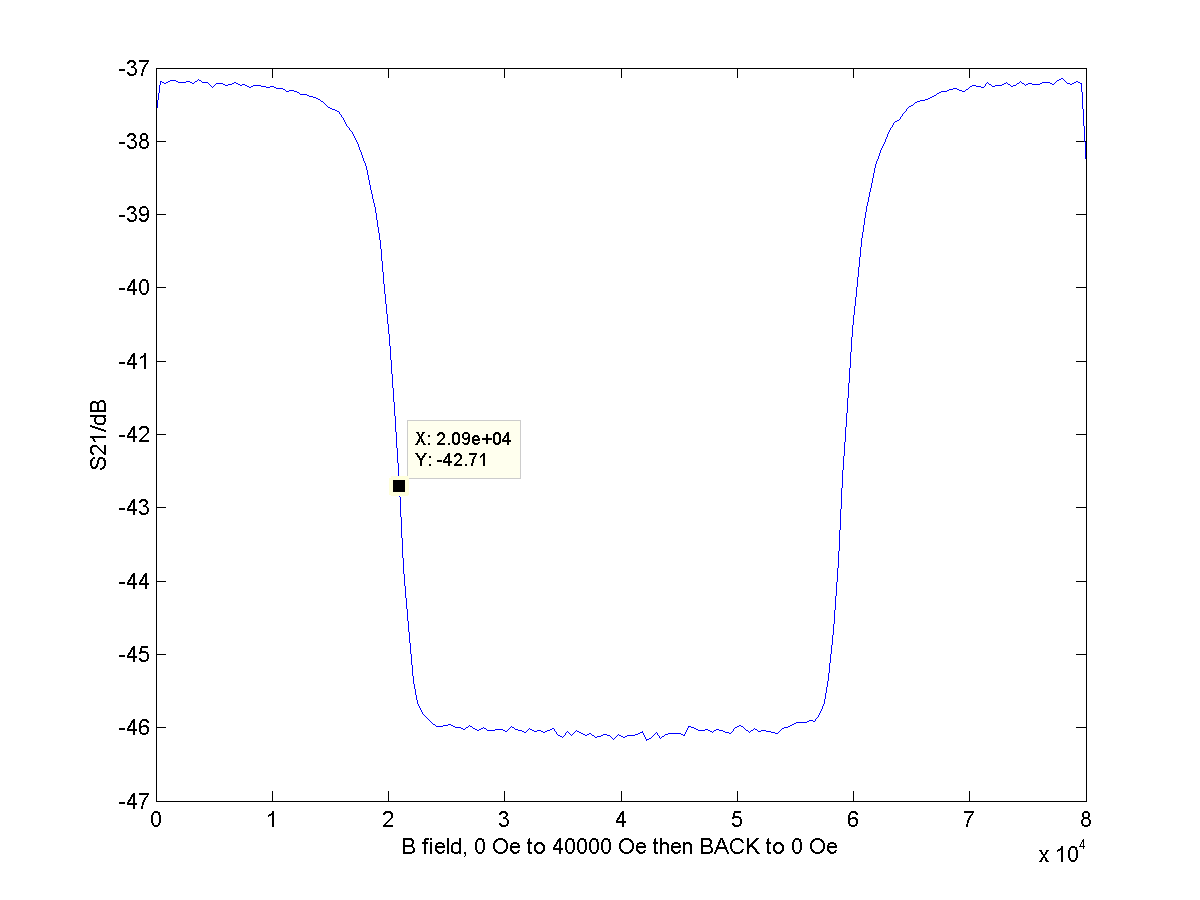
\includegraphics[width=3.2in]{figures/meas/Test_S_vs_B_20170517T112932.png}
    % \caption{第二个小图形,注意这个图略矮些。subfigure中同一行的子图在顶端对齐。}
  \end{subfigure}
  \caption{PPMS磁场与VNA频率扫描}
  \label{fig:PPMSTestFieldSweep}
\end{figure}

                  通过扫描磁场可以看出,测试器件的临界磁场在$2。09\times 10^4$Oe,也即约2T。对于谐振腔模式在磁场变化下的变化规律,我也观察到了和文献中类似的频率移动与品质因子变化的现象,并且与磁场扫描的方向有关\cite{Song2009,Bothner2012}。由于现象较为复杂,不在此处进行讨论。


                        
                  % subsection 磁场扫描 (end)
            % section 测量系统测试 (end)










            \section{样品托的设计与改进} % (fold)
            \label{sec:样品托的设计与改进}

            由孙麓岩研究组郭星翰同学设计的样品托如图\ref{fig:oldSampleBox}所示,由盖子与底座组成。在测量系统使用过程中,我发现了一些问题并想出了一些解决方案,对样品托进行了改进。

\begin{figure}[h]
  \centering%
  \begin{subfigure}{0.4\textwidth}
    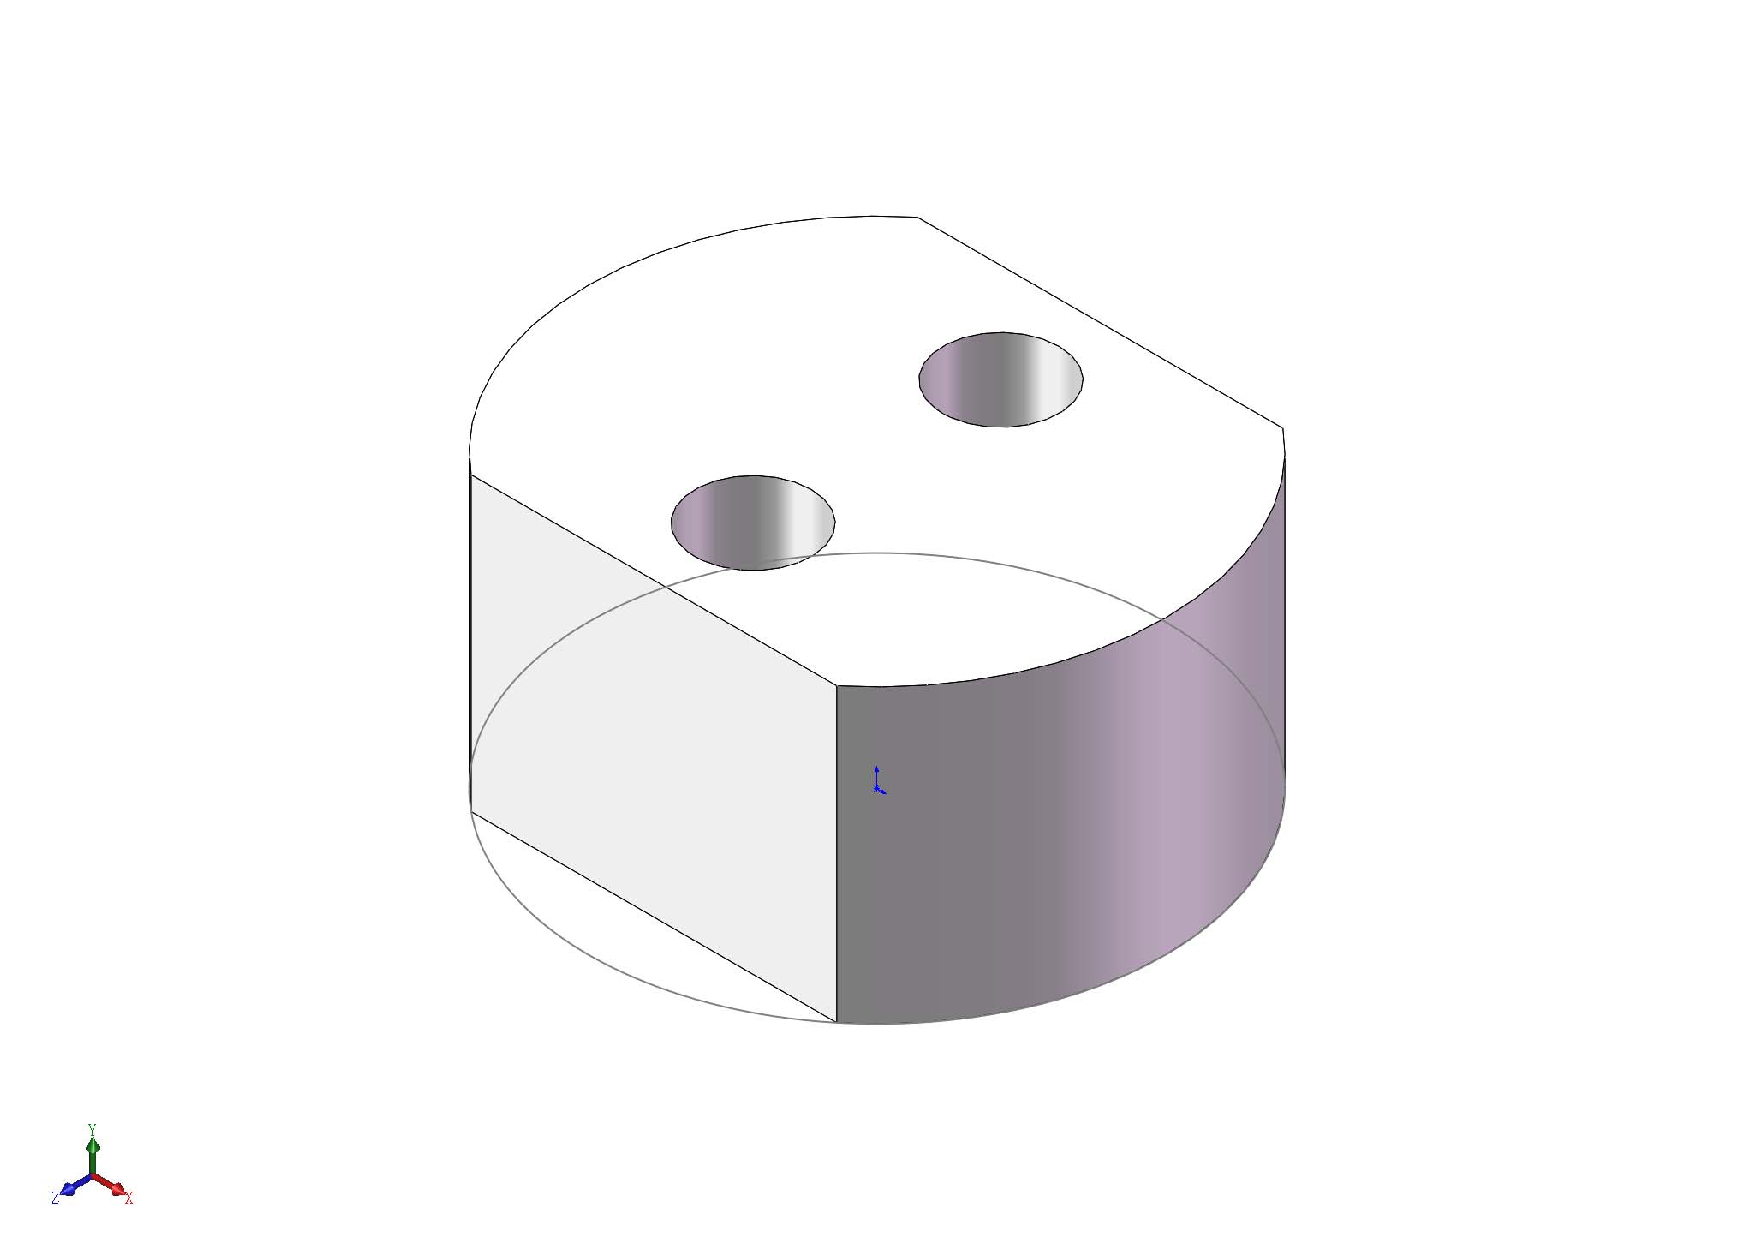
\includegraphics[width=2.2in,angle=270]{Smallbox1.pdf}
    % \caption{第一个小图形}
  \end{subfigure}%
  % \hspace{4em}%
  % \hspace*{\fill}
  \begin{subfigure}{0.4\textwidth}
    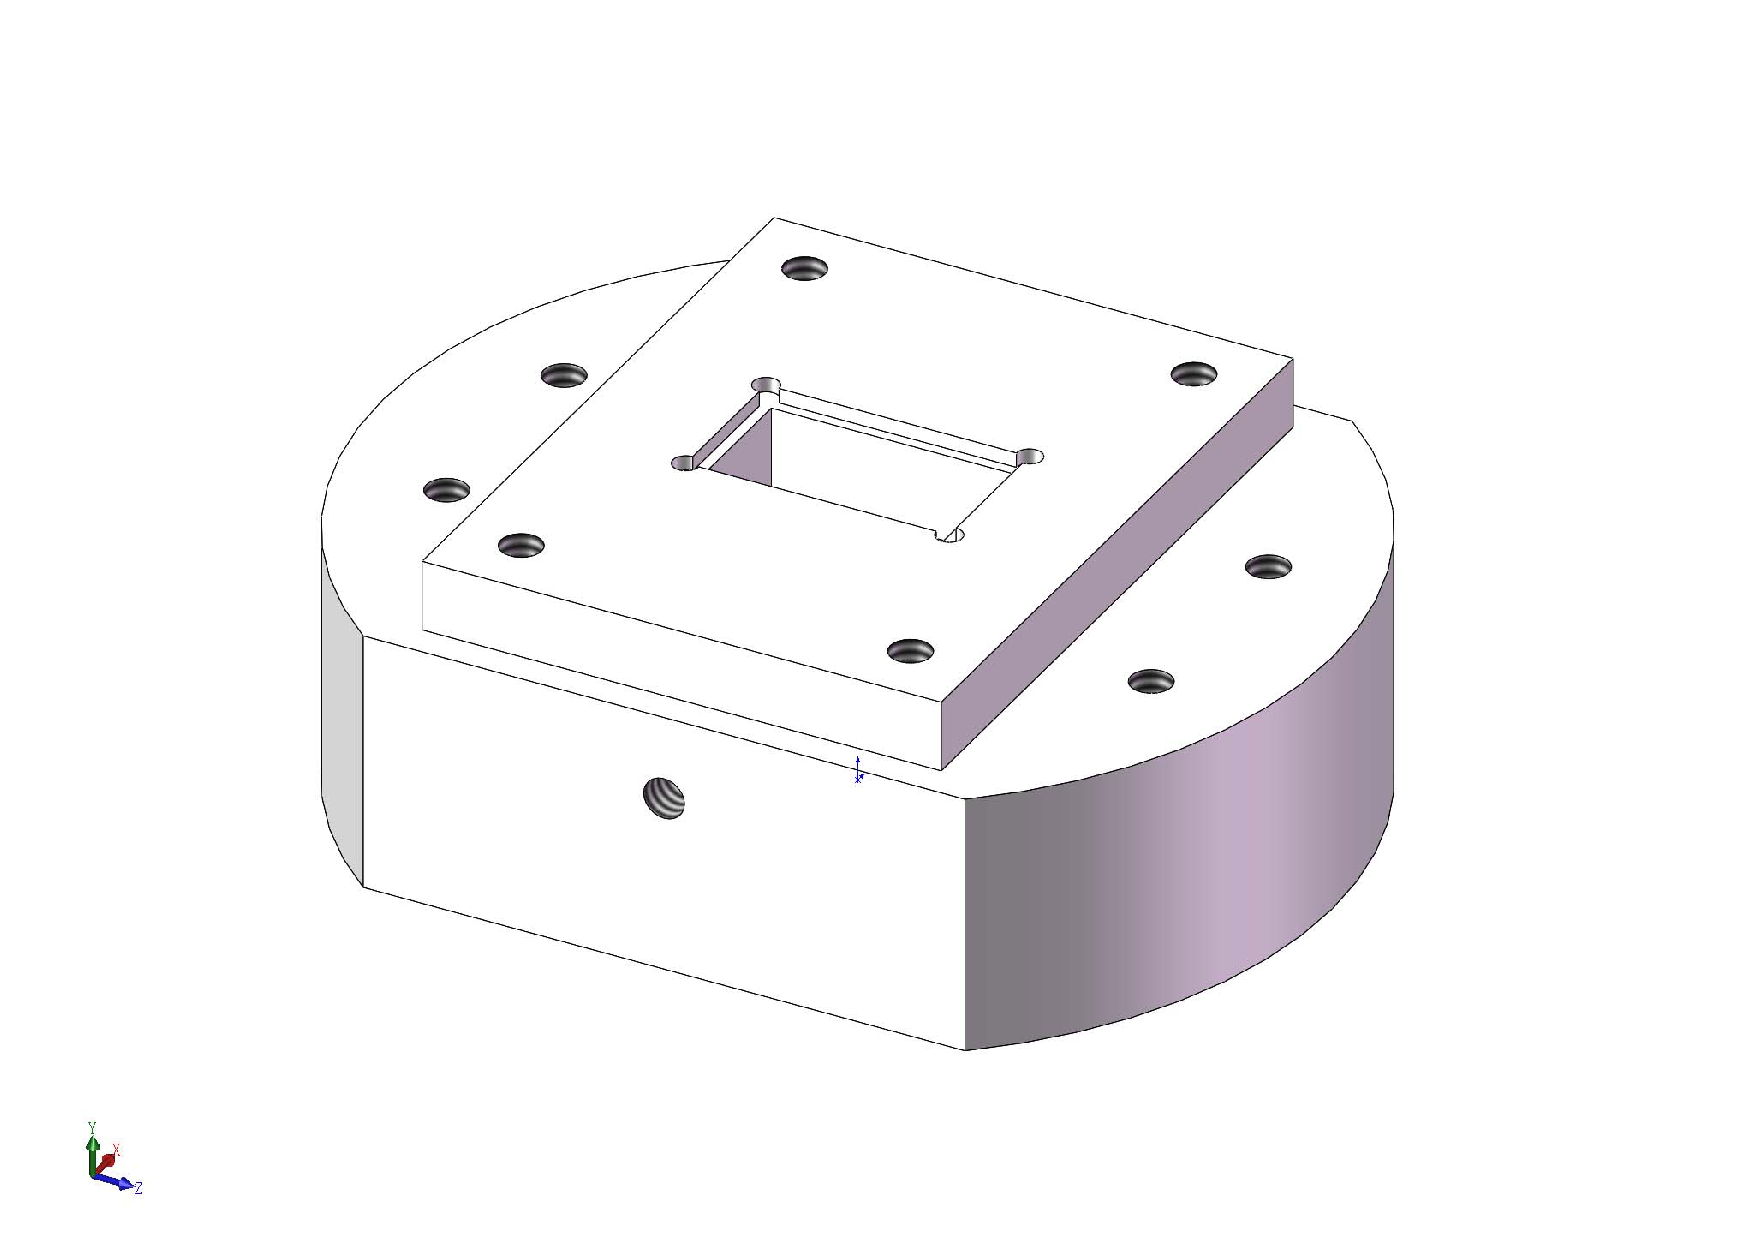
\includegraphics[width=2.2in,angle=270]{Smallbox2.pdf}
    % \caption{第二个小图形,注意这个图略矮些。subfigure中同一行的子图在顶端对齐。}
  \end{subfigure}
  \caption{原有样品盒盖子与底座设计}
  \label{fig:oldSampleBox}
\end{figure}


            在现有的样品托中,微波信号经同轴传输线通过盖子上的两个圆孔,再经过SMP转PCB的接头垂直转至PCB板上的平面波导上,再通过点焊的连接转入器件上的平面波导中。样品座放置样品的位置下方有方形空洞,一方面为尽可能排除样品盒自身的谐振模式,另一方面为减小样品盒与样品间的电容,从而使得样品上微波出入端的cross talk尽量小\cite{Wenner2011}。现有样品托使用的转接头为Rosenberger~19S102-40ML5。另一个可能可以改进的地方为,样品托的盖子与底座通过螺丝固定,螺丝右下至上穿过底座与盖子固定,不便安装。在实际使用中,四个螺孔往往只会用到两个。因此,在改进的设计中,螺丝改为从上至下安装,且数目减少为两个,如图\ref{fig:newSampleBox}所示。



\begin{figure}[h]
  \centering%
  \begin{subfigure}{0.4\textwidth}
    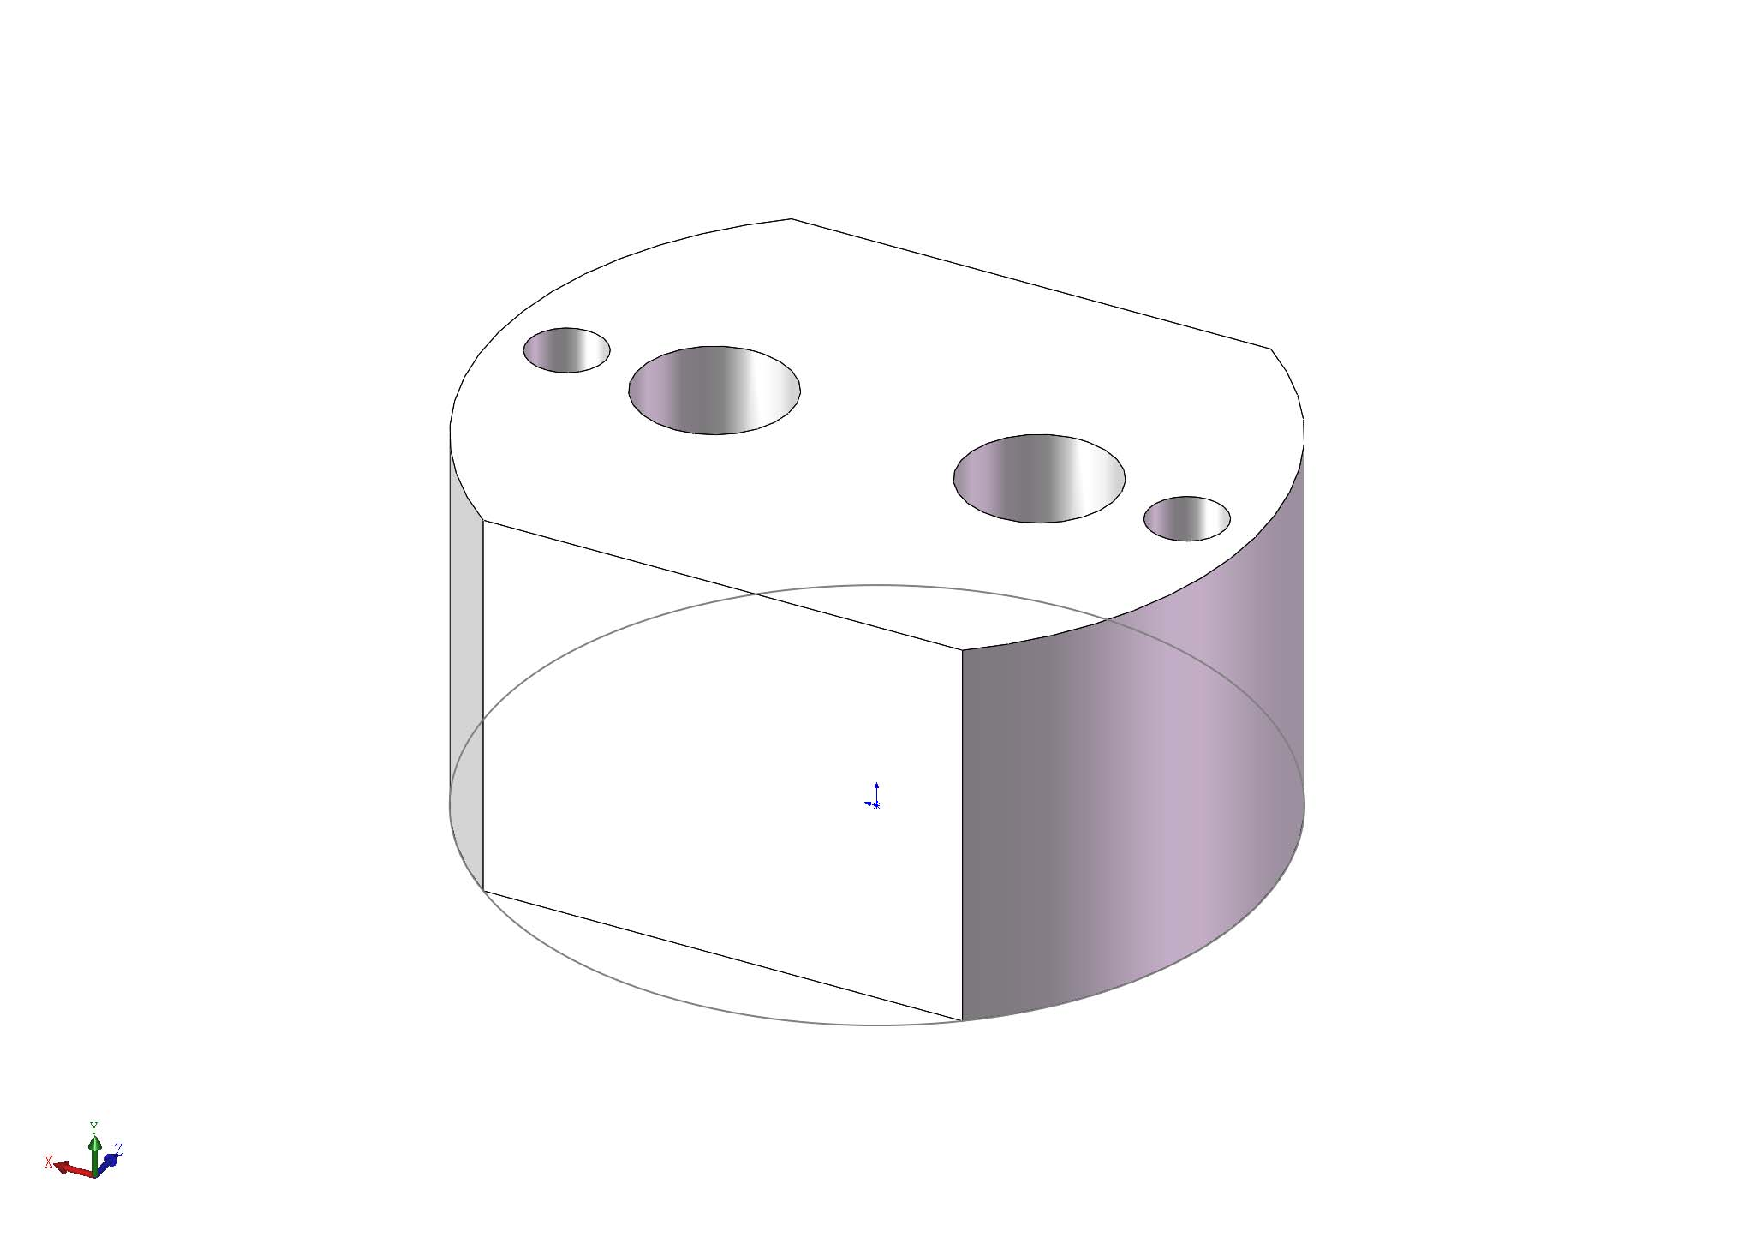
\includegraphics[width=2.2in,angle=270]{SmallboxCover.pdf}
    % \caption{第一个小图形}
  \end{subfigure}%
  % \hspace{4em}%
  % \hspace*{\fill}
  \begin{subfigure}{0.4\textwidth}
    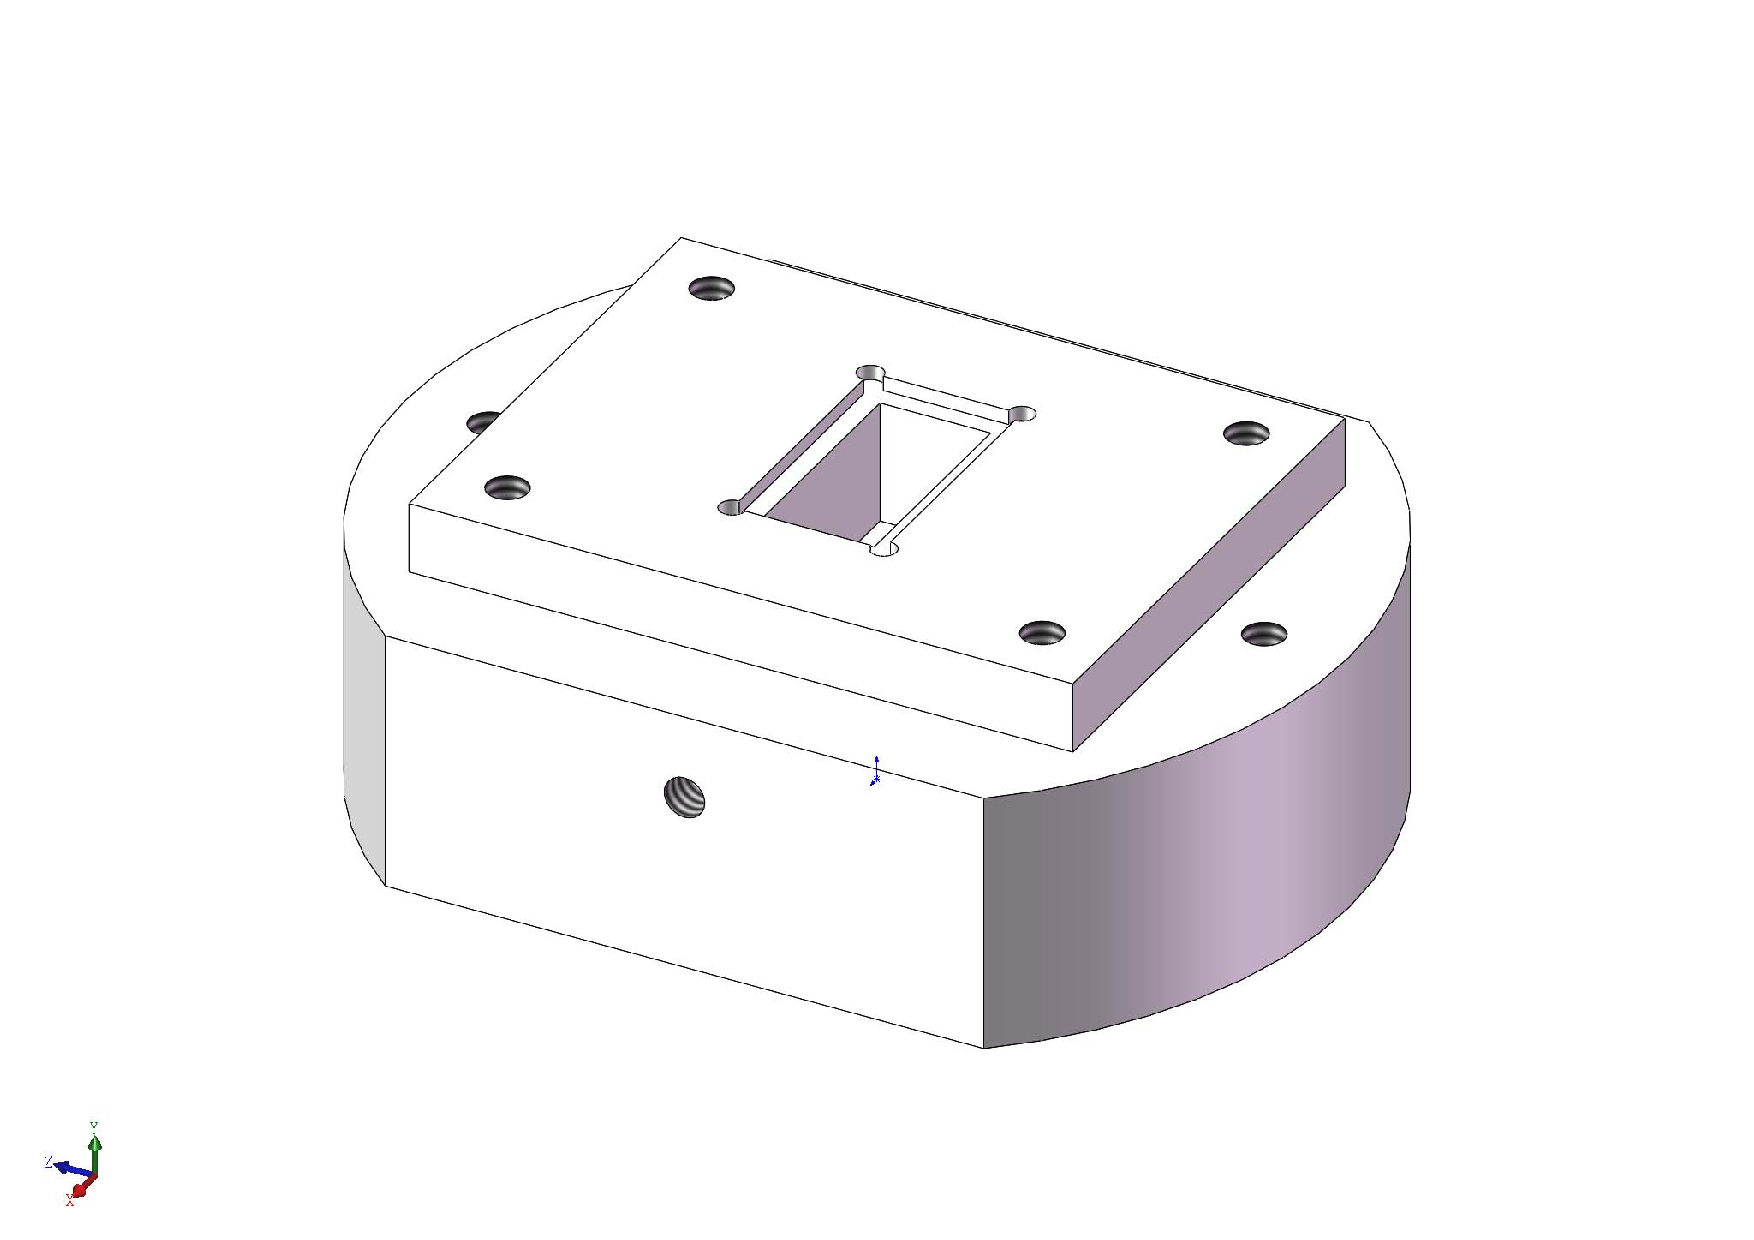
\includegraphics[width=2.2in,angle=270]{SmallboxHolderHori.pdf}
    % \caption{第二个小图形,注意这个图略矮些。subfigure中同一行的子图在顶端对齐。}
  \end{subfigure}
  \caption{改进后样品盒盖子与底座设计}
  \label{fig:newSampleBox}
\end{figure}


            另一个较大的改进为竖直装样。在第\ref{sec:测量系统概述}中已经提到,我们希望样品也能够竖直放置,因此需要设计新的样品托底座。样品托的盖子通过SMP接头固定在样品杆上,拆卸与更换相对不便,因此我希望设计出能够同时供水平放样的底座与竖直放样的底座使用的样品盖。竖直放样的样品座的大致设计思路为,将现有的样品座竖直剖分为两部分,在剖分的竖直面上即可安装新的光刻板与样品。因此,需要更换SMP转接头,并根据新的转接头设计PCB板,并且使转接头的位置与水平放样时一致,以便同时使用相同的样品盖。


            具体设计时,考虑到了点焊时器件需能够很好的水平放置,因此采用平行于样品底座两侧平面的方向将原有样品做剖分,这样点焊时器件与新的底座能够平稳放置。而这样剖分底座,将导致微波接头位于剖分面与原有样品底座表面的交线方向上,与原有微波接头排列方向垂直。因此为配合新的底座对应的样品盖,水平放置器件的样品底座也需更改PCB与器件的放置方向,如图\ref{fig:newSampleBox}所示,通过简单旋转原有样品底座的PCB板部分,使得原有的PCB板设计与已经制作出了并焊接上SMP接头的PCB板仍旧能够继续使用。

            通过研究SMP转接头型号,我们确认所需的新的转接头为Rosenberger~19S202-40ML5-NM。我根据现有SMP接头与PCB板尺寸,以及将会采用的新SMP接头的尺寸,设计了拆分后的样品底座与盖子设计,如图\ref{fig:newVertiSampleBox}所示。


\begin{figure}[h]
  \centering%
  \begin{subfigure}{0.4\textwidth}
    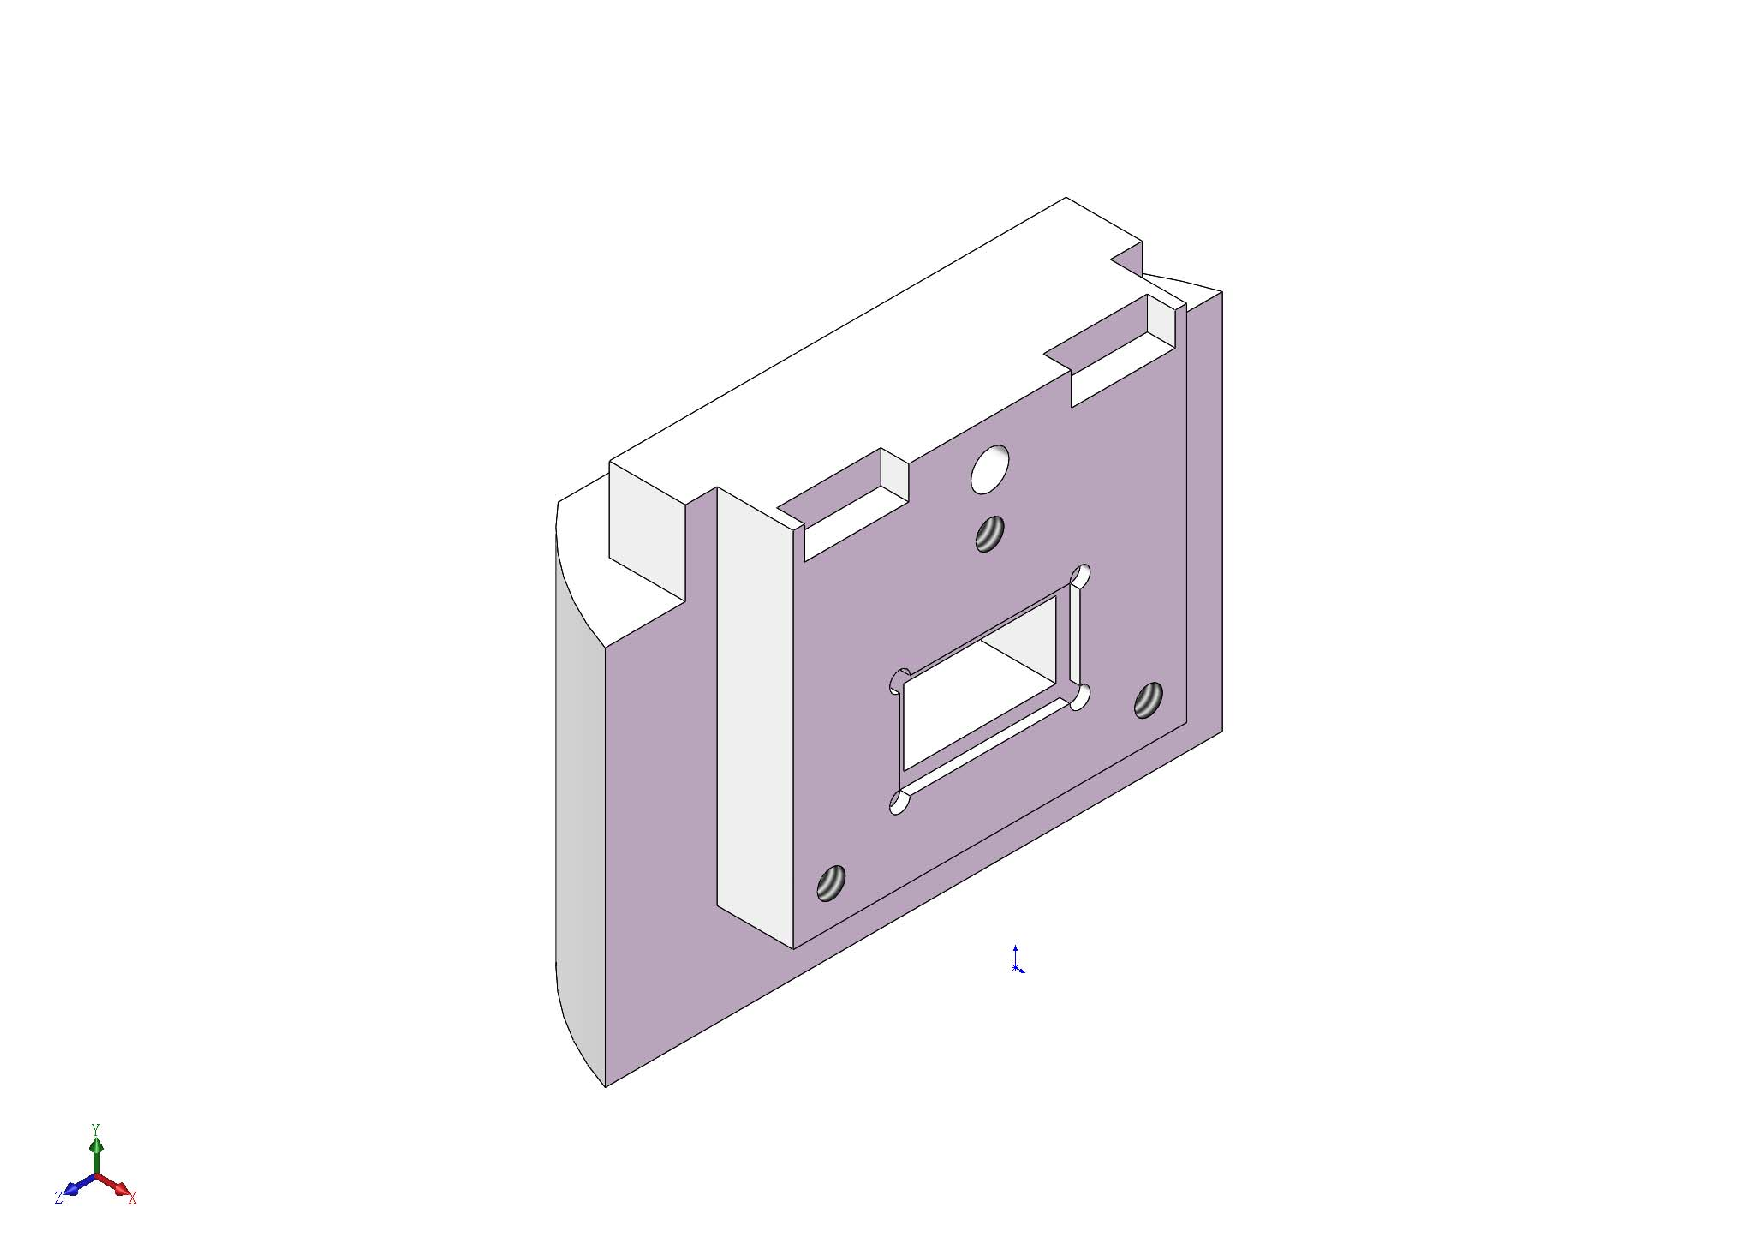
\includegraphics[width=2.2in,angle=270]{SmallboxHolderVertTotalHolder.pdf}
    % \caption{第一个小图形}
  \end{subfigure}%
  % \hspace{4em}%
  % \hspace*{\fill}
  \begin{subfigure}{0.4\textwidth}
    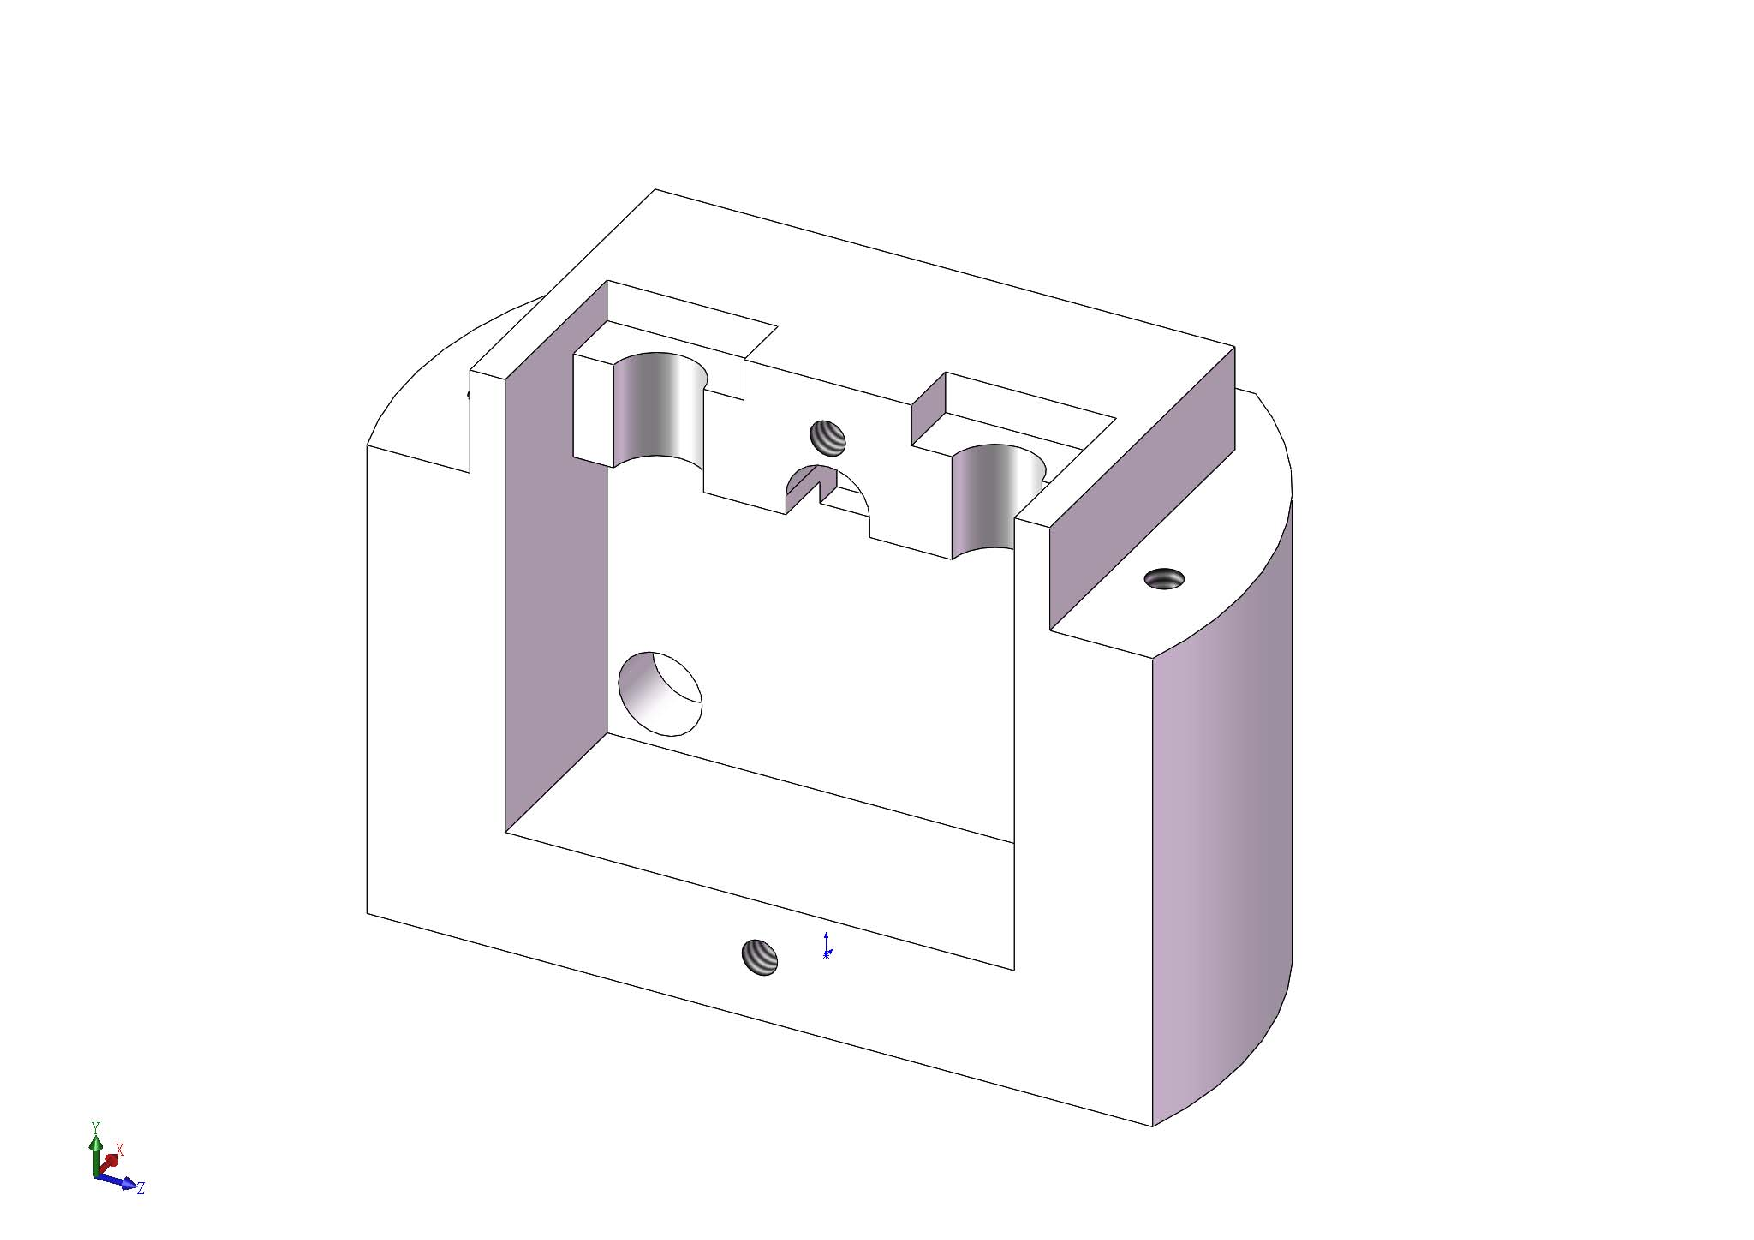
\includegraphics[width=2.2in,angle=270]{SmallboxHolderVertTotalCover.pdf}
    % \caption{第二个小图形,注意这个图略矮些。subfigure中同一行的子图在顶端对齐。}
  \end{subfigure}
  \caption{为竖直放样品所所设计的样品盒底座拆分出的盖子与底座设计}
  \label{fig:newVertiSampleBox}
\end{figure}


            其中的底座部分参考了原有水平放羊的底座的设计通过凸台使得盖子能够更好的封闭样品所在的空间。放置样品的部分下方有方形空洞,四角留出空间便于去除样品。新的样品座设计对应的PCB板的设计如图\ref{fig:SmallboxHolderVertTotalHolderPCBV2}所示。PCB板的上边沿左右两侧将各焊接一个SMP接头,将微波信号耦合进PCB板上的平面波导中。另一个改进为在PCB与器件通过点焊连接的部分对传输线的中心线进行了放大,便于进行点焊,可与原有的图\ref{fig:PPMSSetupTestChip}中的PCB设计进行对比。
                  


\begin{figure}[h]
  \centering%
  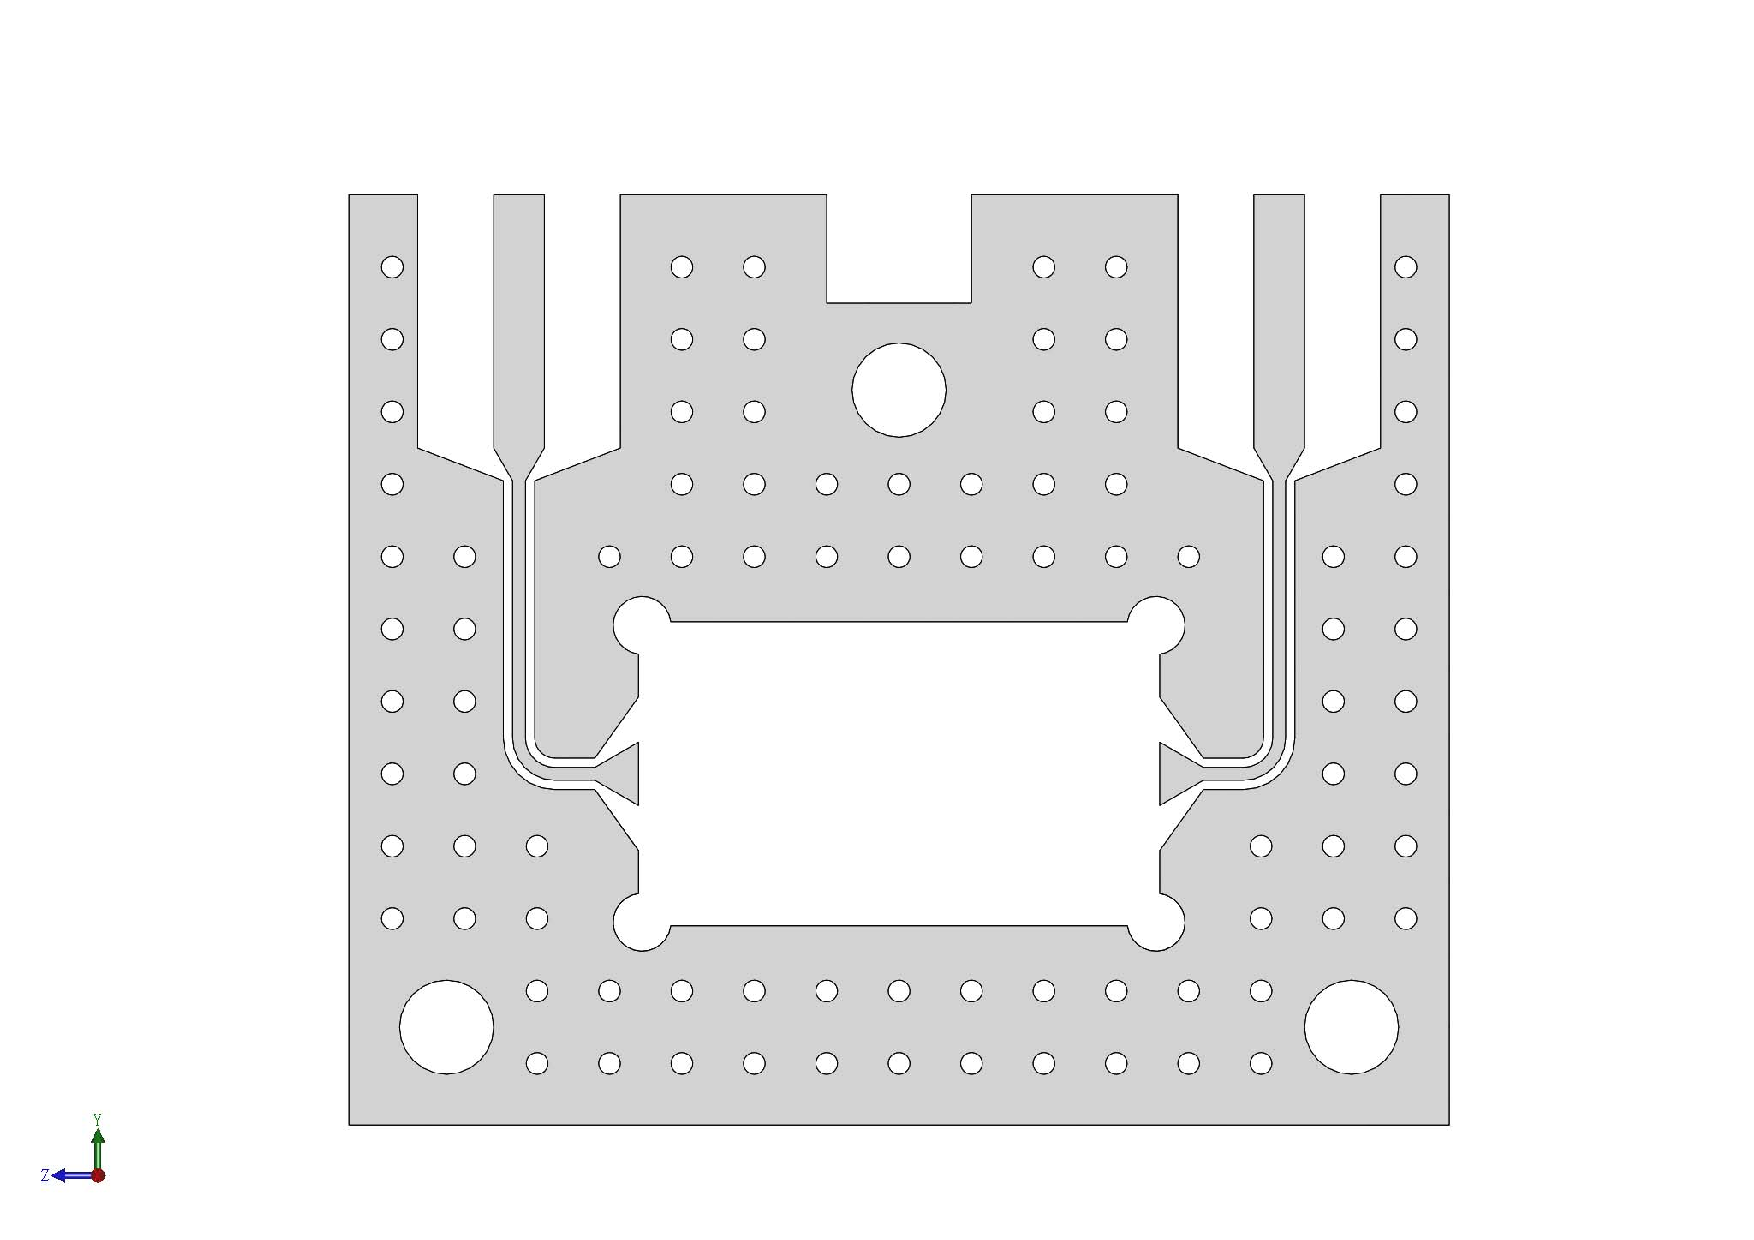
\includegraphics[width=5in,angle=270]{SmallboxHolderVertTotalHolderPCBV2.pdf}
  \caption{为新的竖直放置样品的样品盒所设计的PCB板}
  \label{fig:SmallboxHolderVertTotalHolderPCBV2}
\end{figure}






            % section 样品托的设计与优化 (end)




